\documentclass{article}
\usepackage[paperheight=17.2cm,paperwidth=32.2cm,margin=0cm]{geometry}
\usepackage{tikz}
\usepackage{pgfplots}
\usetikzlibrary{calc,arrows,arrows.meta,shapes,spy}
\usepackage{adjustbox}
\usepackage{tikz-dimline}


\begin{document}
	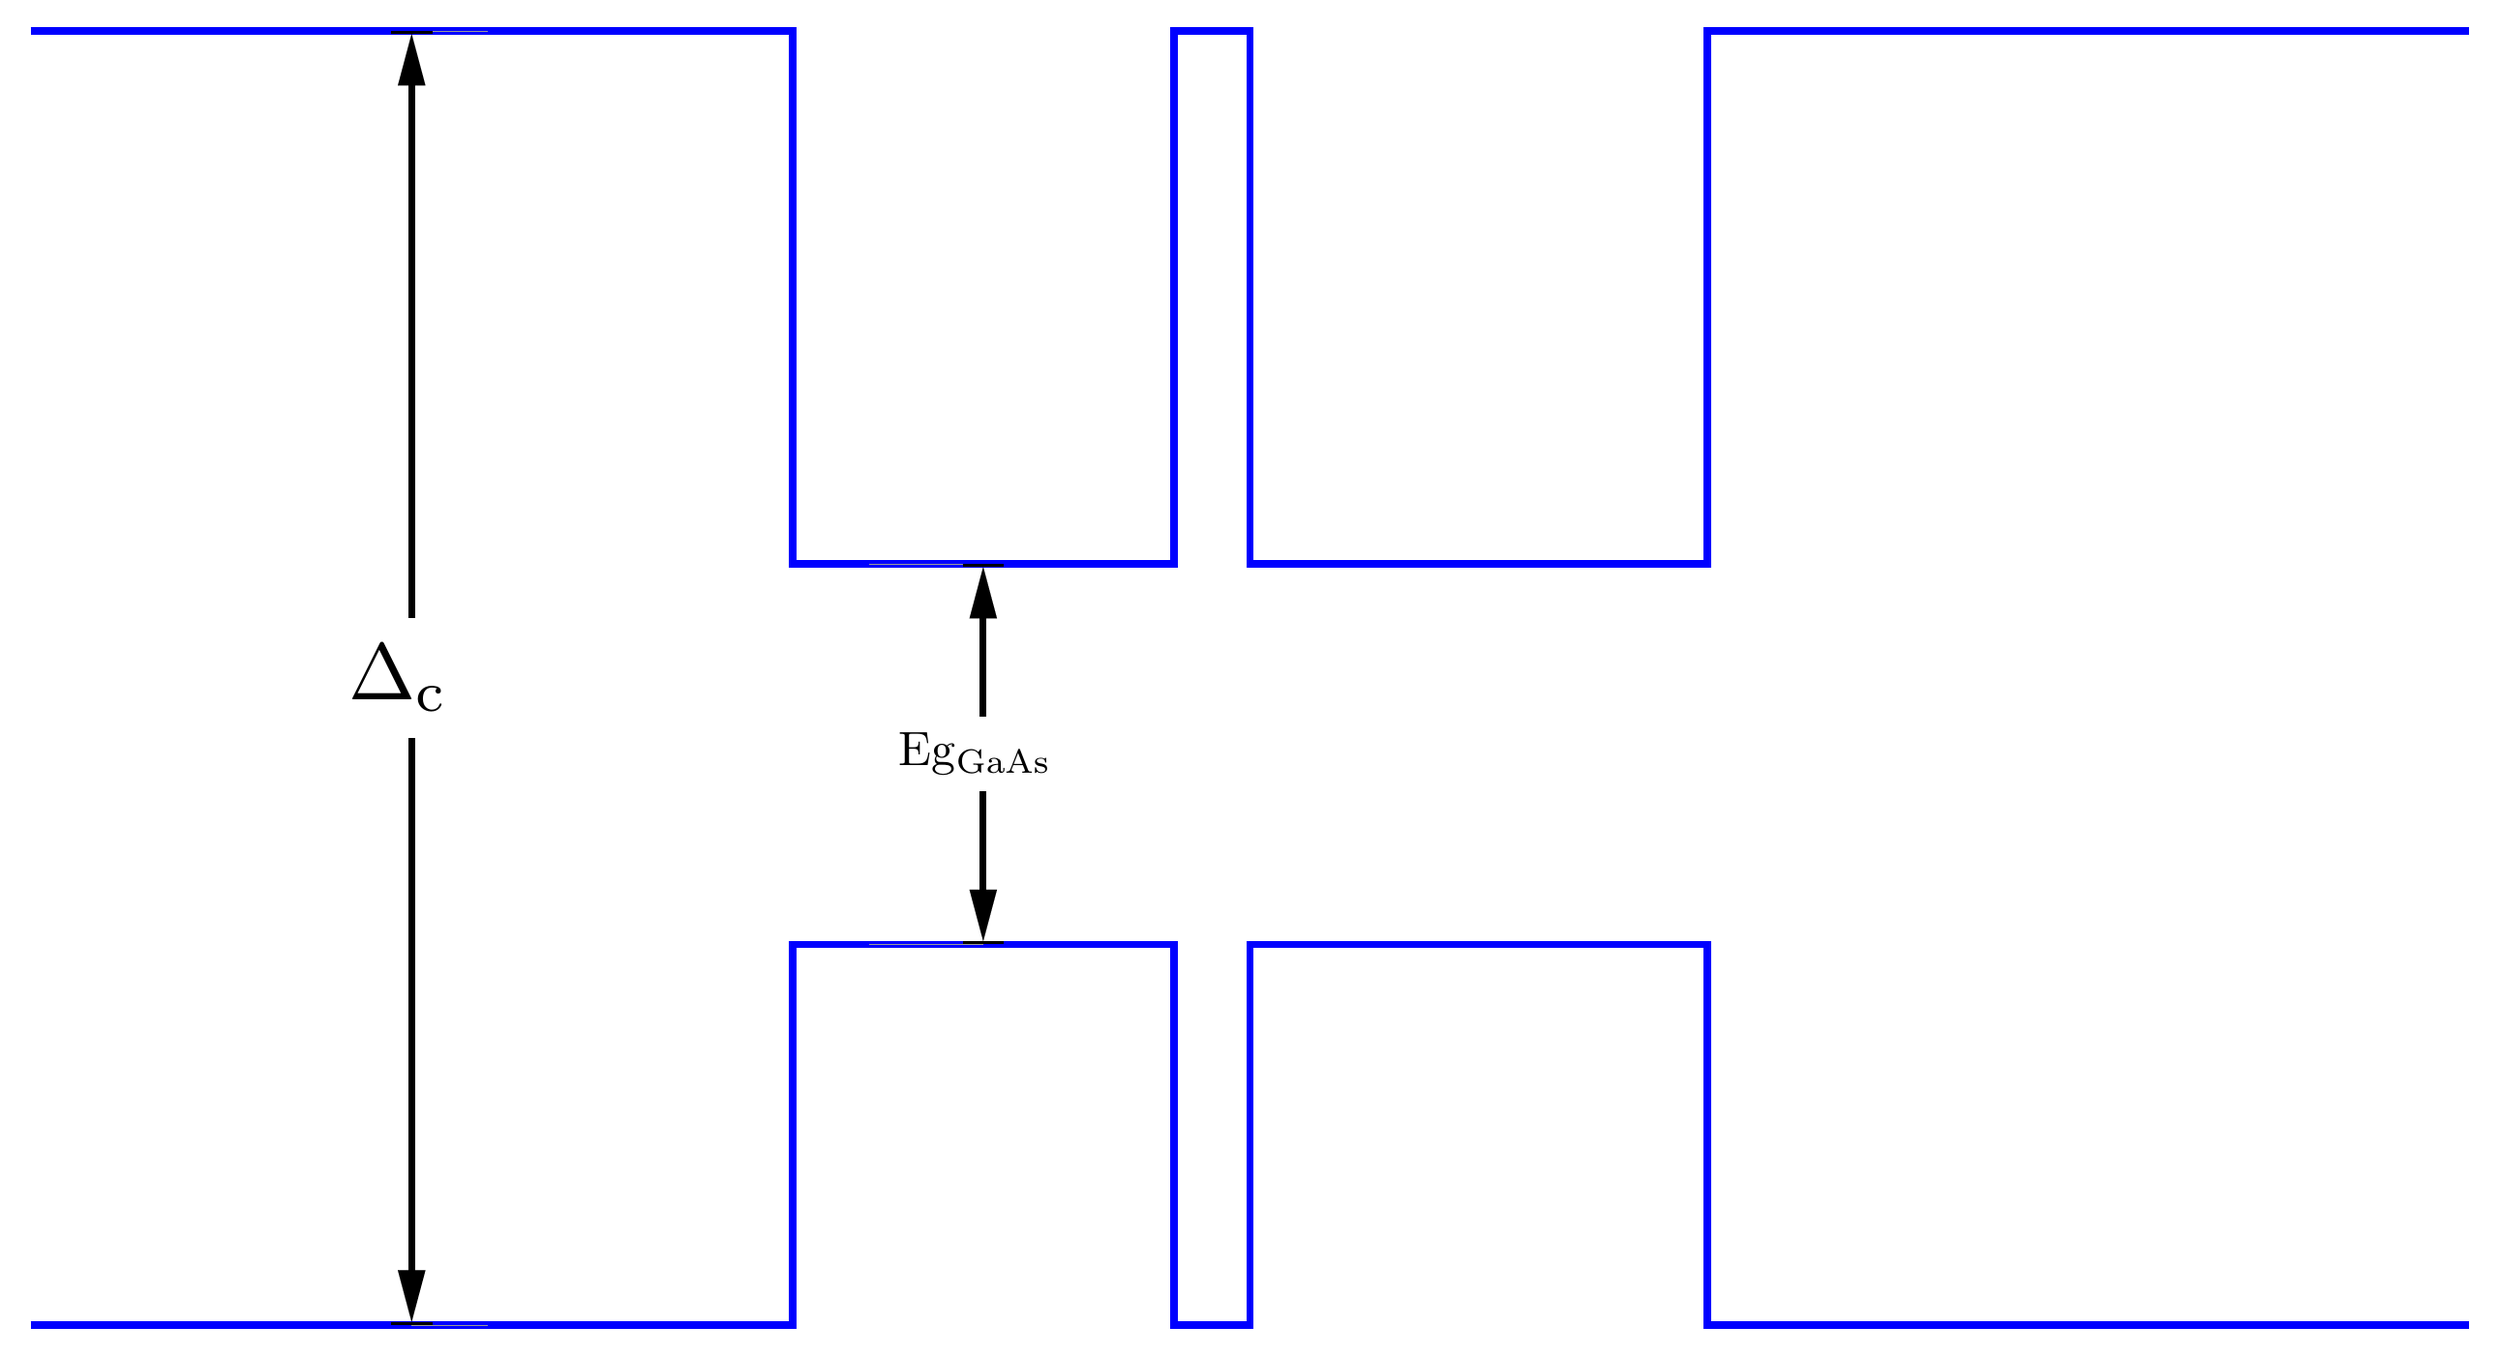
\begin{tikzpicture}
		\draw[line width=1mm,blue] (0,0)--(10,0)--(10,5)--(15,5)--(15,0)--(16,0)--(16,5)--(22,5)--(22,0)--(32,0);
		\draw[line width=1mm,blue] (0,17)--(10,17)--(10,10)--(15,10)--(15,17)--(16,17)--(16,10)--(22,10)--(22,17)--(32,17);
		%\filldraw[gray,opacity=0.5] (0,0)--(10,0)--(10,17)--(0,17);
		%\filldraw[yellow!70!white,opacity=0.5](10,5)--(15,5)--(15,10)--(10,10);
		%\filldraw[gray,opacity=0.5] (15,0)--(16,0)--(16,17)--(15,17);
		%\filldraw[yellow!70!white,opacity=0.5](16,5)--(22,5)--(22,10)--(16,10);
		%\filldraw[gray,opacity=0.5](22,0)--(32,0)--(32,17)--(22,17);
		
		%\draw[{Stealth[scale=3]}-{Stealth[scale=3]}] (12.5,5)--(12.5,10);
		%\node[scale=2] at (13.75,7.5) {$\mathrm{Eg_{GaAs}}$};
		
		
		\dimline[color= black,
		line style = {line width=0.9mm},
		extension start length=-0.3, 
		extension end length=-0.3,
		label style = {rotate=-90,midway,scale=1.8,fill=white},
		] { (12.5,5)}{(12.5,10)}{$\mathrm{Eg_{GaAs}}$ };
		
		
		\dimline[color= black,
		line style = {line width=0.9mm},
		%extension start length=-0.3, 
		%extension end length=-0.3,
		label style = {rotate=-90,midway,scale=3,fill=white},
		] { (5,0)}{(5,17)}{$\mathrm{\Delta_c}$ };
	\end{tikzpicture}
\end{document}



